\documentclass[10pt]{beamer}

% theme
\usetheme{PaloAlto}
\usecolortheme{spruce}
\setbeamertemplate{navigation symbols}{}

% packages
\usepackage{hyperref}
\usepackage{graphicx}

% attributes
\title{\textbf{ExaMA WP3 -- Dashboard Performances}}
\author[Tanguy PIERRE]{Tanguy Pierre\\[1cm] \small{Supervisors: V. Chabannes, J. Cladellas}}
\institute{University of Strasbourg}
\date{9th of April}


% **********************  START  **********************
\begin{document}

\frame{\titlepage}


\begin{frame}
    \frametitle{\textbf{Project description}}

    \begin{itemize}
        \addtolength{\itemsep}{10pt}
        \item Part of the \textit{ExaMA} project
        \item Benchmarking is for:
        \begin{itemize}
            \item performances comparison
            \item transparency about the evaluation process
            \item references in order to avoid performance decline
            \item data analysis depending on context
        \end{itemize}
        \item {\footnotesize\url{https://feelpp.github.io/benchmarking/benchmarking/index.html}}
    \end{itemize}
    \begin{figure}
        \centering
        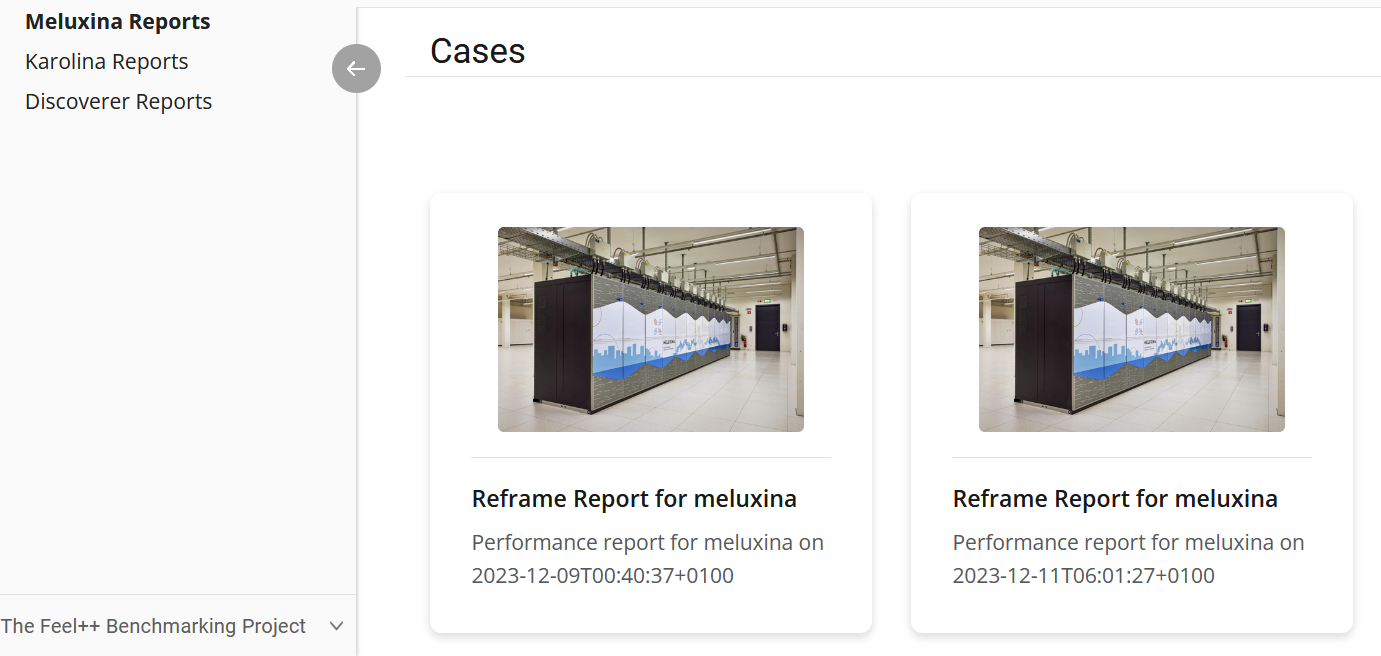
\includegraphics[width=0.8\textwidth]{../../illustrations/feelpp-dashboard.png}
      \end{figure}
\end{frame}

\begin{frame}
    \frametitle{\textbf{Tools}}
    \begin{itemize}
        \addtolength{\itemsep}{10pt}
        \item \textit{ReFrame HPC}, a framework allowing system's complexity abstraction in order to focus only on the algorithm's performance
        \item \textit{Feel++}, a C++ library for Galerkin methods
        \item \textit{Antora}, a documentation site generator \small(\textit{.adoc} to \textit{.html})
        \item \textit{Plotly}, the well-known data visualization library
    \end{itemize}
    \begin{figure}
        \centering
        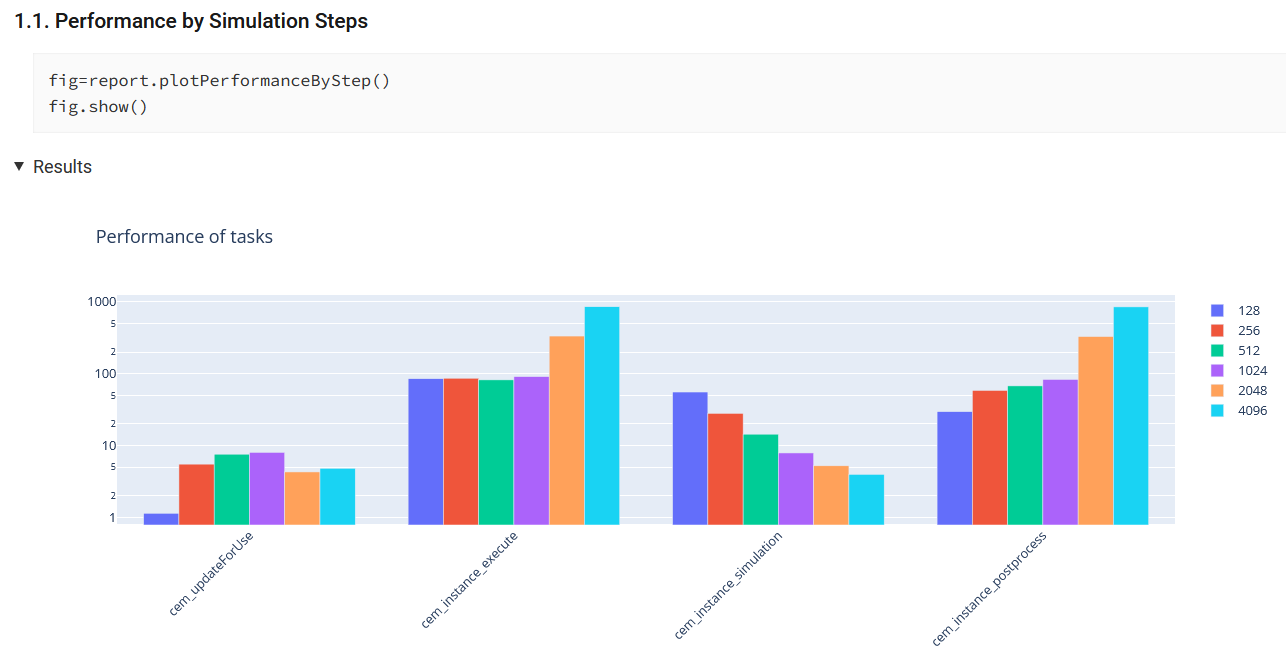
\includegraphics[width=0.8\textwidth]{../../illustrations/benchmarking-graphics.png}
      \end{figure}
\end{frame}


\begin{frame}
    \frametitle{\textbf{Objectives}}
    The necessary resources for publishing results are already available:
    Python scripts for reading ReFrame results and reporting them to an AsciiDoc file.\\
    As it as repetitive task, our objectives are as follows:\\
    [10pt]
    \begin{itemize}
        \addtolength{\itemsep}{10pt}
        \item Establish a workflow based on:\\
                [0.2cm]
                \textbf{Continuous Integration / Continuous Deployment}
        \item Database creation for easy access and retrieval of results\\
        [1cm]
    \end{itemize}
    The initial focus will be on heat-related algorithms from the Feel++ library.\\
\end{frame}


\begin{frame}
    \frametitle{\textbf{Roadmap}}
    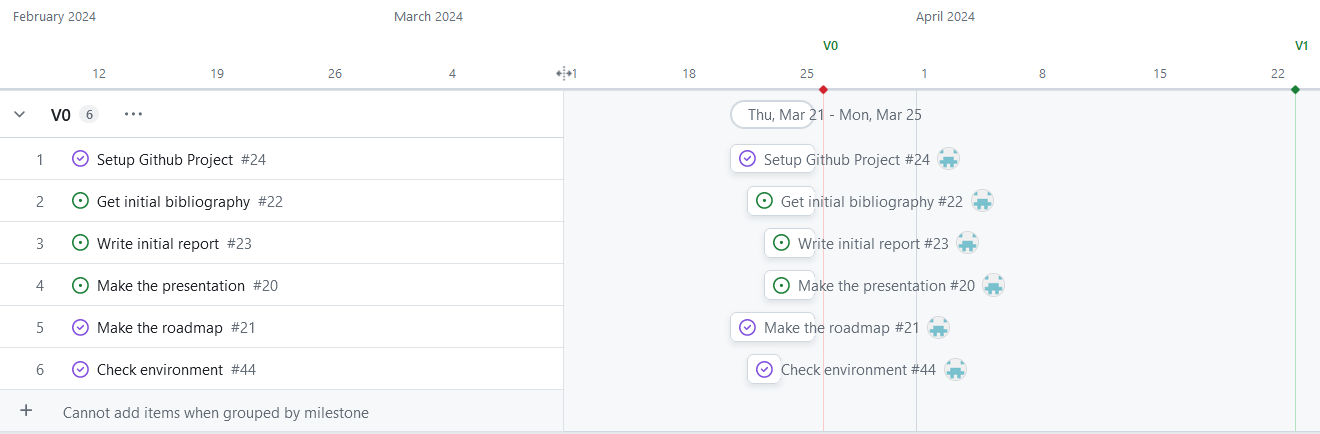
\includegraphics[width=\textwidth]{../../roadmap/roadmapv0-group.png}\\
    [1cm]
    Only generic conducting issues, except from environment checking.\\
    More precise project-relative issues and objectives have to be defined for V1.
\end{frame}


\end{document}